\documentclass[oneside]{book}
\usepackage[utf8]{inputenc}
\usepackage{graphicx}
\usepackage{geometry}
\usepackage{float}
\usepackage{textcomp}
\usepackage{gensymb}
\usepackage{amsmath}
\usepackage{listings}
\geometry{portrait, margin=1. in}
\usepackage[colorlinks = true,
            linkcolor = blue,
            urlcolor  = blue,
            citecolor = blue,
            anchorcolor = blue]{hyperref}

\lstset{language=Python}
\lstset{frame=lines}
%\lstset{caption={Insert code directly in your document}}
%\lstset{label={lst:code_direct}}
\lstset{basicstyle=\footnotesize}



\usepackage{color}

\definecolor{dkgreen}{rgb}{0,0.6,0}
\definecolor{gray}{rgb}{0.5,0.5,0.5}
\definecolor{mauve}{rgb}{0.58,0,0.82}

\lstset{frame=tb,
  language=Java,
  aboveskip=3mm,
  belowskip=3mm,
  showstringspaces=false,
  columns=flexible,
  basicstyle={\small\ttfamily\color{blue}},
  numbers=none,
  numberstyle=\tiny\color{gray},
  keywordstyle=\color{blue},
  commentstyle=\color{dkgreen},
  stringstyle=\color{mauve},
  breaklines=true,
  breakatwhitespace=true,
  tabsize=3,
  %rulecolor=\color{blue},
  %backgroundcolor=\color{darkgray}
}


\begin{document}

\begin{titlepage}
\begin{center}
 {\huge\bfseries SubMIT Off Campus Resources\\}
 % ----------------------------------------------------------------
 \vspace{1.5cm}
 {\Large\bfseries Put Authors Here et. al.}\\[5pt]
 robertej@mit.edu\\
 \href{https://latexonline.cc/compile?git=https\%3A\%2F\%2Fgithub.com\%2Frobertej19\%2FSubMITDocs\&target=main.tex\&command=pdflatex\&trackId=1594872205396}{Live Document Location}\\[14pt]
  % ----------------------------------------------------------------
 \vspace{2cm}


% {By}\\[5pt] {\Large \sc {Me}}
 \vfill
 % ----------------------------------------------------------------

 \vfill
{June 2020}
\end{center}
\end{titlepage}

\tableofcontents

%\chapter{Meetings}
%    \href{https://bluejeans.com/7572697578}{Meeting Link} \quad \quad
\href{https://latexonline.cc/compile?git=https\%3A\%2F\%2Fgithub.com\%2Frobertej19\%2FSubMITDocs&target=main.tex&command=pdflatex&trackId=1591043936822}{Overleaf Online Location}
\section{Thursday May 28 2020}
    \subsection*{Python Versions}
        \indent We discussed that SubMIT only has python 2.6.6 and has not yet disclosed plans to upgrade / install python3. It was decided to try and write the code to work with python3 as much as possible as it works fine on OSG, SubMIT isn't used much presently, and python2.6 has security flaws.
    \subsection*{Other Notes}
        \indent Mauri and Bobby continue to try to work out python bindings with htcondor.
    





\section{Thursday June 4 2020}
    \subsection*{Using Right Python Path and Modules}
        which python returns /apps/bin/python\\
        need to explicitly use /usr/bin/python2 to get htcondor module to work. I tried changing what "python2" does in bashrc but was getting error messages\\
        /usr/bin/python2 -- this works\\
        /usr/bin/python3 -- no module named 'pytz' (needed for utils/utils.unixtimeconvert()\\
        python2 -- no module named "htcondor"\\
        python3 -- no module named "htcondor"\\

    \subsection*{gemc-jsonify footer issue}
        \begin{figure}[H]
        \centering
        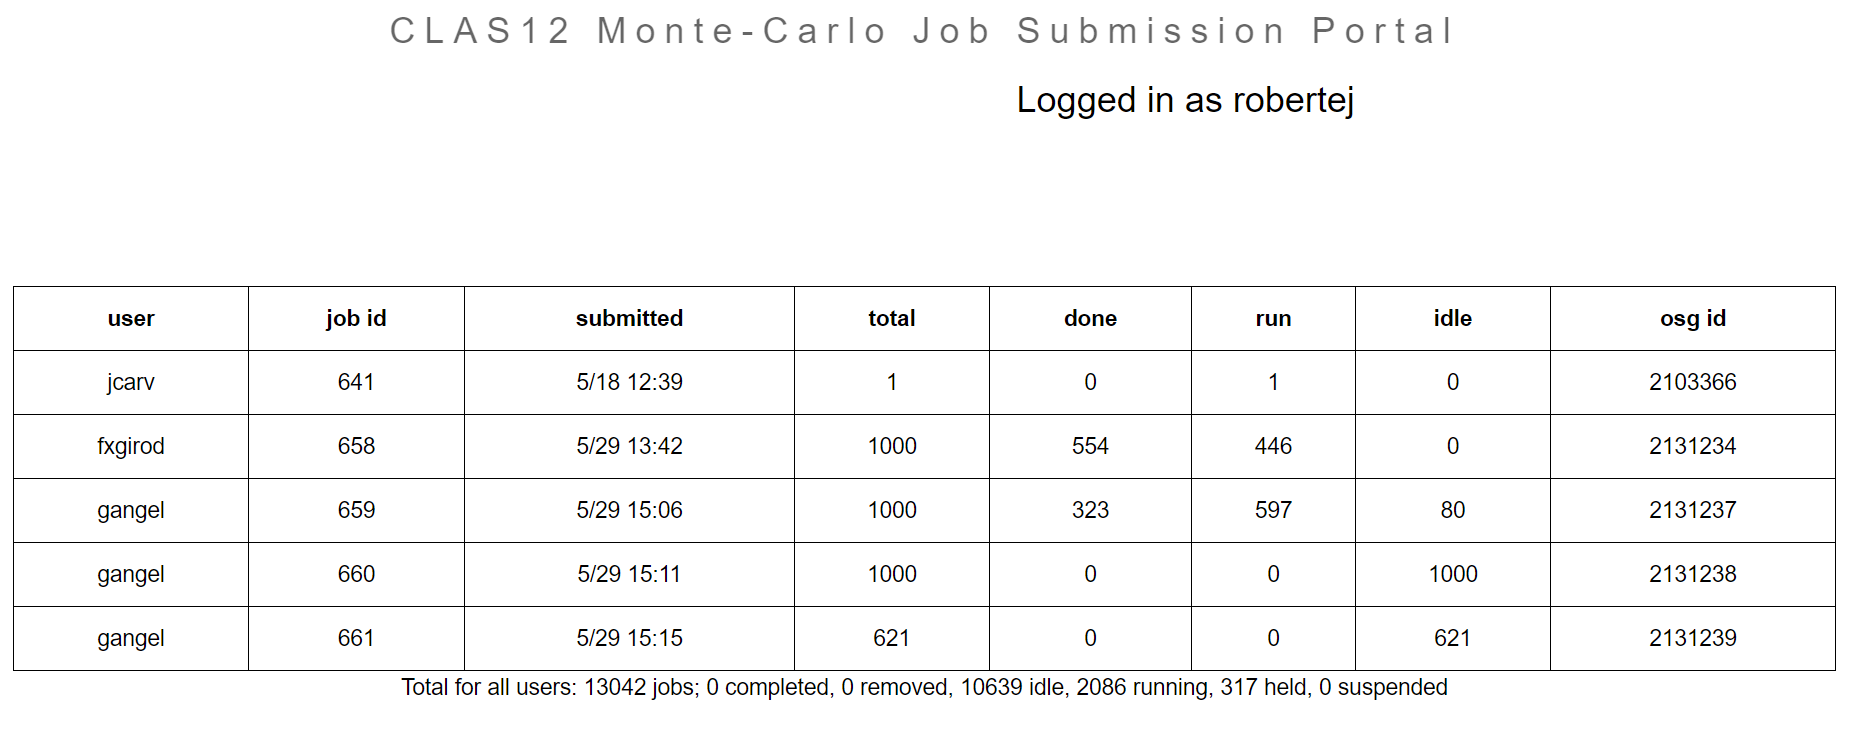
\includegraphics[scale=0.5]{Meetings/20200604/files/jobs-total.PNG}
        \caption{GEMC Web Portal Stats Table Example}
        \label{fig:my_label}
        \end{figure}

    
    Footer metadata - all jobs is for all jobs from JLab, not just CLAS12, this isn't very useful?
    
    \subsection*{Error Handling for when code breaks}
    Error handling: How do we want to handle this? Cant exactly print to screen. Want to send emails when things are breaking? Write to log? something else?
           
    
    \subsection*{Other}
    Are we still indending to put all hard coded variables into FS.py?\\
    Does an up to date Schema diagram for DB exist?\\
    any way to turn off bell in ssh terminal on ifarm? Can't edit /etc/config\\
    
    















\section{Thursday Jan 21 2021}
    \subsection*{Organization}
    \begin{itemize}
        \item Tasks List
        \item Communication channels (Slack / Teams)
        \item Meeting times
        \item AoB
    \end{itemize}
    
    
connect farm with OSG guys - give mauri a contact
TUESDAY 2 PM Next meeting - meet every other week
farm sees networkhas singularity and also have cvmfs

how to dedicate jobs to MIT
send mauri specific name of cluster

streamline code, put into one repository
create repositoryto do document - put a text filedocumentation and manualREADMEinternal documentation for developerssubdirectory for documentation of files
coordinate with jlab it?monitoring job failures

Send Email to Mauri about nodes at MIT

    
%This section needs work to compile correctly    
%\chapter{Tasks}
%    Have room for held
Email set up
Both total jlab and gemc jobs
add “clas12” total to the “all total”
b. add priority to JSON (not to be used on normal production page, just the test page)


need to rewrite hashmap as class
see if need to combine scard and kwargs
put priority and held in 

parse_scard in scard_helper.py is not really doing anything?


I think scard is just read in as raw text, and then parsed out on server side?


******************move setup database and configure args to a different file from SubMIT.py. scard_handler seems not useful. 





Need to include Held jobs in listing?

Incorportate Travis-CI

Top task: Python bindings: 

\href{https://htcondor.readthedocs.io/en/latest/apis/python-bindings/}{htcondor python bindings}


Automatic generation and usage of container – dependent quantities such as generator lists, configuration files

How is prority defined?

Automatic generation and usuage of experiment – dependent quantities such as background merging file list 


Background merging mechanism


Support multiple containers


Add more control over job flow, output sturcture

Set up Contintious integration



If genOutput is changed to “dvcs.dat” from “dvcsgen1.dat", everything is fine
In the new web_interface I didn’t even include all those generators for this reason. Also, soon we should have the scard object to remove those maps in the fs.py that have the hardcoded names.



) Using online repositoris:
	2.1) Create documentation to describe how to set up online repositories
	2.2) Is there a way to store things the other computer has acress to bypass the internet, maybe on volitle? It can be a pain to upload to remote online repositories. Could we upload to 	github?
Move connect_to_db to utils/utils
Add sqlite option to utils/jsonify_logfile.py



1) Is there a way to get information about what version of gemc / what other versions of the software are in the CVMFS image (which is distributed to all systems, Im guessing?)
	1.1) see what gcards are avaliable?
	1.2) Add way to specifiy specific gcard within docker containe




How will we log the number of events / the number of jobs if the user supplies the gcards / LUND files?
use log output files to monitor job submissions




5.) Work on fixing -w issue -- should not have to use, also gcards should be downloaded on node



2.)
Set up a dynamic list of gcards acceptable 
have list returned to user on what gcards are valid, can assume clas12.gcard & a description of what gcard is / does / has in it


Regarding the gcards, I think it's ok to have them in a file for now. We can wait a few container releases to see if what's in the file matches the container content or it has to be different. 
The command to retrieve the list from the container is straightforward:

singularity exec --home ${PWD}:/srv --pwd /srv --bind /cvmfs --contain --ipc --pid /cvmfs/singularity.opensciencegrid.org/jeffersonlab/clas12simulations:production ls /jlab/work/ | grep gcard


    
%This section needs work to compile correctly    
\chapter{Structure}
    

\href{https://gemc.jlab.org/web_interface/index.php}{GEMC web interface}

\href{https://github.com/mit-mc-clas12}{Github Source}

Priority handling:  This is the way we handle priority P , which is basically P =  (constant) / N Running Jobs

   (depends on the output of 1).
    

\chapter{Usage}
    \section{MySQL Commands}
    For all command examples, we are using the hostname of "jsubmit.jlab.org", the username of "robertej". Substitute these values for your needs. N.b. SQL has a formalism where all commands are capitalized and all items are lower cased. We will try to stick to that in all examples but note that SQL is actually case insenstitive as a language. Also, the language must end each command in a semicolon. \\
    
    
    \subsection{Connecting to Database}
        To establish an interactive session on the command line:
        \begin{lstlisting}
            mysql -h jsubmit.jlab.org -u robertej -p 
        \end{lstlisting}
        
        If you don't want to have an interactive session, or don't want to enter a password each time, you can pass a configuration file as:
        
        \begin{lstlisting}
            mysql --defaults-extra-file=msql_conn.txt     
        \end{lstlisting}
        
        Where mysql\_conn.txt is a text file of the form:
        
        \begin{lstlisting}
            [client]                                                                                            
            user='robertej'                                                                                                   
            password='realpassword'
            host='jsubmit.jlab.org'
            database='CLAS12OCR' 
        \end{lstlisting}
    
    \subsection{Basic MySQL Commands}
    
        See available databases:
        
        \begin{lstlisting}
            SHOW DATABASES;
        \end{lstlisting}
        
        Create a databases:
        
        \begin{lstlisting}
            CREATE DATABASE CLAS12OCR;
        \end{lstlisting}
        
        Delete a databases:
        
        \begin{lstlisting}
            DROP DATABASE CLAS12OCR;
        \end{lstlisting}
        
        Enter a particular database:
        
        \begin{lstlisting}
            USE CLAS12OCR;
        \end{lstlisting}
        
        See available tables in a database:
        
        \begin{lstlisting}
            SHOW TABLES;
        \end{lstlisting}
        
        See schema of a particular table:
        
        \begin{lstlisting}
            DESCRIBE CLAS12OCR.users;
        \end{lstlisting}
        
        Leave the interactive MySQL environment:
        
        \begin{lstlisting}
            EXIT;
        \end{lstlisting}
    
    \subsection{Advanced MySQL Commands}
    
    How to see size of databases (copy verbatim):

        \begin{lstlisting}
            SELECT table_schema "DB Name",
                    ROUND(SUM(data_length + index_length) / 1024 / 1024, 1) "DB Size in MB" 
            FROM information_schema.tables 
            GROUP BY table_schema; 
        \end{lstlisting}
    
    How to dump all information from a database into a text file:
    
    \begin{lstlisting}
        mysqldump -h jsubmit.jlab.org --skip-comments --skip-extended-insert -u robertej -p CLAS12OCR > test10.sql  
    \end{lstlisting}
    
    The two skip options are optional and only include information extraneous to the actual data in the database. They can be omitted without error.\\
    
    How to make a copy of a database to another MySQL DB:

    \begin{lstlisting}
        mysqldump -h jsubmit.jlab.org -u robertej -p CLAS12OCR | mysql -h jsubmit.jlab.org -u robertej -p CLAS12OCRBackup
    \end{lstlisting}    
    
    \subsection{Common MySQL Commands in CLAS12OCR}
    
        Get list of all users and current running jobs:
        
        \begin{lstlisting}
            SELECT user, total_running_jobs FROM users;
        \end{lstlisting}
        
        More usefully, see the 10 most recent submissions on the database:
        
        \begin{lstlisting}
            SELECT user, client_time, run_status FROM submissions ORDER BY user_submission_id DESC LIMIT 10;
        \end{lstlisting}
        
        
        If you want to wrap everything all up in one, you can do: 
        \begin{lstlisting}
        mysql --defaults-extra-file=msql_conn_test.txt -N -s --execute='select user, client_time, run_status from submissions ORDER BY user_submission_id DESC LIMIT 10;' 
        \end{lstlisting}
        
        
        How to copy runscript from the database to a text file:
        \begin{lstlisting}
        mysql --host jsubmit.jlab.org --user='username' --password='password' --database='CLAS12OCR' --execute='SELECT runscript_text FROM Submissions WHERE submissionID = 1; ' > example.txt
        \end{lstlisting}

    \subsection{Permissions in MySQL}
    This section is yet to be populated
    \iffalse
    mysql permissions:
    show users:
    
    select user, host from mysql.db where db='CLAS12OCR';
    
    show grants:
    
    show grants for 'clas12jserver'@'%.jlab.org';
    
    GRANT ALL ON . TO 'clas12jserver'@'%.jlab.org';
    
    current users that access the db:
    
    show processlist;
    
    \fi

\section{Testing with SQLite}
    \subsection*{Create SQLite DB}
        \begin{lstlisting}
            python utils/create_database.py --lite=name.sql
        \end{lstlisting}
    
    \subsection*{Submit job on client side to SQLite DB}
        \begin{lstlisting}
            python client/src/SubMit.py --lite=name.sql -u=username client/scard_type1.txt
        \end{lstlisting}
        
        
         sqlite run to download the running script and the gcard. Assuming DB is in the same dir
    \begin{lstlisting}
        sqlite3 CLAS12_OCRDB.db "SELECT runscript_text FROM
        Submissions WHERE submissionID = $submissionID"  > $nodeScript
    \end{lstlisting}
    
\section{Statistics and Logging}
    \subsection*{GEMC JSON Web Interface Statistics}
         To test on sqlite that things work as intended: 
         \begin{lstlisting}
            python3 utils/gemc_json_logging.py -lite=CLAS12OCR.db -t -o testoutput.log
        \end{lstlisting}
        ~\\
        \newline
        Normal use (with no arguments, default will use mysql db and output to osgLog.json)
        \begin{lstlisting}
            python3 utils/gemc_json_logging.py 
        \end{lstlisting}


\section{Using Travis-CI}
    \href{https://travis-ci.org/}{Travis Location}
    
    Important parts of Travis CI:\\
    There are currently documents important for Travis CI:\\
    
    .travis.yml\\
    requirements.txt\\
    travis.sql\\
    travis\_tests.py\\
    readtests.py\\
    
    \subsection{.travis.yml}
        
        \begin{lstlisting}
        
            language: python
            python:
              - "2.7"
            #  - "3.6"      # current default Python on Travis CI
            # command to install dependencies
            services:
             - mysql
            before_install:
             - mysql -u root --password="" < test/travis.sql
            # - echo "USE mysql;\nUPDATE user SET password=PASSWORD('devpassword') WHERE user='dev';\n" | mysql -u root
            install:
            #  - if [[ $TRAVIS_PYTHON_VERSION == 2.7 ]]; then pip install -r req-py2.txt; fi
            # - pip install -r req-py2.txt; python_version == "2.7"
             - pip install -r test/requirements.txt
            # - pip install mysql-python
            # command to run tests
            
            #script: python2 testapp.py || python3 testapp.py #For now, can't get python3 to work properly
            script: python2 test/travis_tests.py
        \end{lstlisting}
    
    This file must be named as ".travis.yml" and must be found in the main repository directory. It is the launching point for the CI tests. Here you can specify which python versions you want to test, what services to install, and which programs to run.
    
    \subsection{requirements.txt}
        This file contains which python modules need to be installed in the virtual environment. If something is missing, travis will throw an error, so its not so difficult to get right.
        
    \subsection{travis.sql}
                \begin{lstlisting}
                    # Create DB
                    CREATE DATABASE IF NOT EXISTS `CLAS12OCR`;
                    CREATE DATABASE IF NOT EXISTS `CLAS12TEST`;
                \end{lstlisting}
                This initializes the MySQL databases
                
    \subsection{travis\_tests.py}
        This creates all the logically structure and is a framework to execute commands. Its not so important to look at unless something is broken. 
        
    \subsection{readtests.py}
        This is the actual location where what commands to be submitted on Travis-CI are actually specified. The current command structure is:
        
                \begin{lstlisting}
                 verify_submission_success = command_class('Verify scard submission success',
                                    ['sqlite3','utils/CLAS12OCR.db','SELECT user FROM submissions WHERE user_submission_id=1'],
                                    'robertej\n')
                \end{lstlisting}        
        
       The structure is a class where the first element is the desired name of the command (user defined), the second is the actual command to execute on the terminal, broken up between spaces, and the third element is what the expected output is from the command. The default is "0" if no output comparison is desired to be made. Travis will fail if a non-zero output is specified and is not observed, even if the command processes successfully. 
    
    






\chapter{Meetings}
    \section{Thursday May 28 2020}
    \subsection*{Python Versions}
        \indent We discussed that SubMIT only has python 2.6.6 and has not yet disclosed plans to upgrade / install python3. It was decided to try and write the code to work with python3 as much as possible as it works fine on OSG, SubMIT isn't used much presently, and python2.6 has security flaws.
    \subsection*{Other Notes}
        \indent Mauri and Bobby continue to try to work out python bindings with htcondor.
    





    
\chapter{Pull Request Notes}
   \section{PR Notes for June 1 2020 PR}
    \subsection*{Overview}
        \indent Replaced jsonify\_logfile.py with gemc\_json\_logging.py, increased usability between python2 and python3, created a few utility functions, developed python-htcondor bindings. 
    
    \subsection{Rework of jsonify\_logfile}
        jsonify\_logfile.py - no longer needed, replaced by gemc\_json\_logging.py (perhaps we can pick a better name)\\
        ~\\
        \textbf{Created New File gemc\_json\_logging.py}\\
        gemc\_json\_logging.py - uses get\_condor\_q.py (described below) to grab data directly from htcondor scheduler, and outputs gemc data which should be able to be read directly into the web interface as before.\\
        Usage:\\
        Testing: python3 gemc\_json\_logging.py -lite=CLAS12OCR.db -t -o testoutput.log\\
        Standard: python3 gemc\_json\_logging.py (with no arguements, defaults will use mysql db and output to osgLog.json)\\
         ~\\
        \textbf{Created New Function get\_condor\_q.py}\\
        utils/get\_condor\_q.py - querys the htcondor system and returns relevant information. Can be expanded to return things like priority, number of jobs held, etc. Should continue to add some data verification and edge case handling.\\
        ~\\
        \textbf{Obsolete functions in osgQuery.sh}\\
        utils/shScripts/osgQuery.sh - no longer need to run condor\_q, script can be changed to just run gemc\_json\_logging.py once it is validated to work properly
        
    \subsection{Other}
         \textbf{Created function utils/utils.unixtimeconvert(unixtimestamp, timezone)}\\
        description: put in a utc unix time stamp and timezone (e.g. 'eastern') get out a local time e..g 5/31 12:19 PM.\\
        ~\\
        \textbf{Changed utils/html\_reader.py}\\
        python2 uses html module HTMLParser and urllib2, python3 uses html.parser and urlopen\\
        added utils/getPythonVersion() function to allow to choose which to import dynamically\\
        ~\\
        \textbf{Moved some hard coded variables to fs.py}
    
\iffalse



\chapter{Resources}
    \section{HTCondor and HTC-Python Bindings}
    \href{http://pages.cs.wisc.edu/~adesmet/status.html}{Status and State Numbers}\\
    \href{https://research.cs.wisc.edu/htcondor/HTCondorWeek2016/presentations/Bockelman_Python-tutorial.pdf}{HTCondor-Python Presentation}\\
    \href{https://research.cs.wisc.edu/htcondor/manual/v8.6/condor_q.html}{Condor\_q Command Documentation}\\
    \href{https://research.cs.wisc.edu/htcondor/mail-lists/}{HTCondor Mailing Lists}\\
    \href{https://htcondor.readthedocs.io/en/latest/apis/python-bindings/index.html}{Python Bindings}\\
    
    Even with the above references, some details remained unclear. Here is a useful mapping from python binding commands to condor\_q outputs:\\
    \newline
    \textbf{job.get("ClusterID")} - we have called this different names, but is in the sql db as osg\_ID\\
    \textbf{job.get("JobStatus")} - returns if job is running /idle. See \href{http://pages.cs.wisc.edu/~adesmet/status.html}{Status and State Numbers} for more.\\
    \textbf{job.get("QDate")} - utc unix timestamp of when the job was submitted.\\
    \textbf{job.get("TotalSubmitProcs")} - total number of jobs submitted. To get the number of jobs done, you must subtract all running and idle jobs from the total jobs, i.e. there does not exist a variable tracking how many jobs are done in the batch submission.\\
    
\section{MySQL and SQLite Resources}
    Currently trying to locate these
    
    
\fi

\end{document}
